\section{Debugger Design}%
\label{section-design} In this section we describe the design of a
visualizer for the ReactiveX (Rx) family of RP libraries to answer RQ2.
Given the findings of RQ1, the requirements for our visualizer are:
\begin{description}
        \itemsep0em
    \item[REQ1]
        Provide overview of Observable flows.  This overview should
        support practices 1 and 2, by graphically representing the
        relations between Observables, such that a complete image is
        given of all Observables and how they interact.
    \item[REQ2]
        Provide detailed view inside flow.  This view should support
        practices 3 and 4 by giving access to both data flow and
        life-cycle events and should be able to show the behavior of a
        operator visually.
\end{description}

To meet those requirements, we propose a visualizer consisting of two
parts:  (1) a Data Flow Graph and (2) a Dynamic Marble Diagram.  The
data flow graph satisfies REQ1, providing a high-level overview, showing
how different flows are created, combined and used, while the marble
diagram satisfies REQ2, offering a more in-depth look into a single
selected data flow showing the contents (in terms of values and
subscriptions) of the flows and can be used to learn the behaviors and
interplay of operators.

\subsection{Data Flow Graph}
\paragraph{Simplified graphs} When running a RP program, Observables
are created that depend on other Observables (their \emph{source}) and
Observers are created to send their values to a defined set of Observers
(their \emph{destination}).  Figure~%
\ref{chaincreate} shows these relations in a graph.  For the simplest of
programs, the relations between the Observables ($ O = {o_1, o_2, o_3} $)
and those between Observers ($ S = {s_1, s_2, s_3} $) share an equally
shaped sub-graph after a reversal of the Observer-edges.  To provide
more overview, we process the graph to merge the two Observable and
Observer sequences together, simplifying it in the process, resulting in
a \emph{Data Flow Graph} (DFG) as in Figure~%
\ref{fiddlesimple}.  The process is simple:  we retain only the
Observer-subgraph nodes, complementing them with the meta data of the
corresponding Observable nodes.  Higher order relations are retained, as
shown in Figure~%
\ref{fiddlehigher}.  Figure~%
\ref{screenshot-mergeAll}B shows the DFG in practice.

\begin{figure}[ht]
    \centering
    \begin{tikzpicture}[->,>=stealth',shorten >=1pt,auto,node
    distance=1.5cm,
                    semithick,scale=0.8, every node/.style={scale=0.8}]
    \tikzstyle{every state}=[] \filldraw (0,2) circle (2pt) node[right]
    {of(1,2,3)} -- (0,1) circle (2pt) node[right] {map(\_ * 2)} -- (0,0)
    circle (2pt) node[right] {filter(\_ < 3)};
\end{tikzpicture}

    \caption{DFG of Figure~%
    \ref{chaincreate}}%
    \label{fiddlesimple}
\end{figure}

\begin{figure}[ht]
    \centering
    \begin{tikzpicture}[->,>=stealth',shorten >=1pt,auto,node
    distance=1.5cm,
                    semithick,scale=0.8, every node/.style={scale=0.8}]
    \tikzstyle{every state}=[] \filldraw (0,2) circle (2pt) node[right]
    {of(1,2,3)} -- (0,1) circle (2pt) node[right] {skip(1)} -- (0,0)
    circle (2pt) node[right] {flatMap(() => inner)};

    \filldraw (-1,1) circle (2pt) node[left] {of(`A', `B')} -- (0,0)
    circle (2pt) node[right] {};

    \filldraw (-0.7,1) circle (2pt) node[left] {} -- (0,0) circle (2pt)
    node[right] {};

\end{tikzpicture}

    \caption{DFG of Figure~%
    \ref{chainhigher}}%
    \label{fiddlehigher}
\end{figure}

\paragraph{Layout} Layout is used to add extra meaning to the graph.  If
multiple subscriptions on the same Observable are created, multiple
flows are kept in the graph and they are bundled together in the
resulting layout.  This is designed to help developers find related
flows.  Also it is easy to see that for example an Observable is reused
many times, hinting a possible performance improvement by sharing the
computation (Rx has special \code{share}-operators to multicast).  The
layout is based on StoryFlow~\cite{liu2013storyflow}, which employs a
hierarchical clustering before ordering the graph in a way to reduce
crossings.  Whereas StoryFlow clusters on physical character location,
we cluster flows per Observable.  Furthermore, StoryFlow supports
interactivity in various layout stages of which we use the algorithms
for \emph{straightening} and \emph{dragging} to support selecting a
specific flow, which is then highlighted, straightened and positioned at
the right in order to match the Marble Diagram, shown for the current
highlighted flow.

\paragraph{Color} Coloring the nodes can be used to identify the same
Observable in multiple places in the graph, as Observables can be reused
in different places of the stream.  For example, in Figure~%
\ref{chainhigher} the \code{inner} Observable is reused twice, which we
denote visually by applying the same color to its two occurrences in the
DFG.

\subsection{Dynamic Marble Diagrams} In contrast to the original
diagrams (Section%
\ref{marblediagram}), we use dynamic diagrams which update live when new
events occur and are stacked to show the data in the complete flow.
This allows the developer to \emph{trace a value back through the flow},
a debug operation which is impossible using a classic debugger.
Handcrafted marble diagrams can use custom shapes and colors to
represent events, but for the generic debugger we use only three shapes:
next-events are a green dot, errors are a black cross and completes are
a vertical line, as shown in Figure~%
\ref{screenshot-mergeAll}C.  For our generic debugger, it is unfeasible
to automatically decide which properties (content, shape and color) to
apply to events, as the amount of events and distinguishing features
might be unbounded.  Instead the event values are shown upon hovering.

\subsection{Architecture} To support the visualization, we design a
debugger architecture consisting of two components:  a host
instrumentation and a visualizer.

The \textbf{Host instrumentation} instruments the Rx library to emit
useful execution events.  Depending on the language and platform,
specific instrumentation is required.  Output of the instrumentation is
a platform and language independent graph like Figure~%
\ref{chainhigher}.  By splitting the instrumentation from the
visualization, the debugger can be used for the complete Rx family of
libraries by only reimplementing the first component.  The communication
protocol for the instrumentation is shown in Table~%
\ref{protocol}. Note that the user never needs to use 
this protocol, it is internal to the debugger.

The \textbf{Visualizer} takes the output of the host instrumentation,
the initial graph, and simplifies it into a Data Flow Graph.  Then it
lays out the Data Flow Graph and provides the debuggers User Interface.
By separating the visualizer, we can safely export generated graphs and
visualize them post mortem for example for documentation purposes.

The components can run in their own environment.  The instrumentation
must run inside the host language, while the Visualizer can use a
different language and platform.

\begin{figure*}
    \begin{annotatedFigure}
        {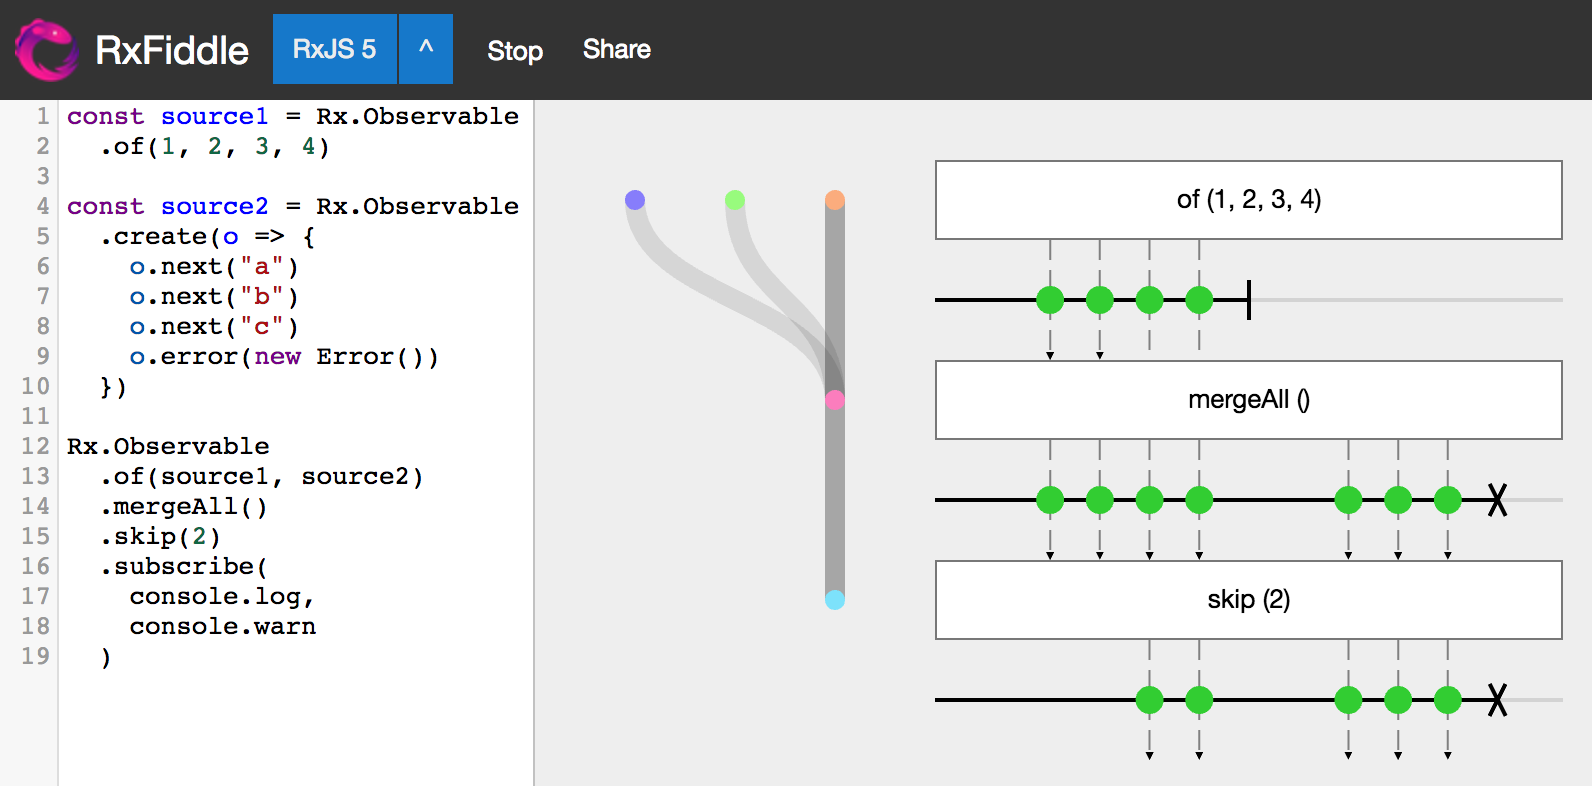
\includegraphics[width=1.0\textwidth]{{images/screenshot.mergeAll2.crop}.png}}
        \annotatedFigureBox{0.039,0.7256}{0.329,0.8716}{A}{0.039,0.1256}%bl
        \annotatedFigureBox{0.363,0.1627}{0.553,0.8248}{B}{0.363,0.1627}%bl
        \annotatedFigureBox{0.568,0.0219}{0.9942,0.8247}{C}{0.568,0.0219}%bl
    \end{annotatedFigure}

    \caption{Screenshot of \href{http://rxfiddle.net/\#type=editor&code=Y29uc3Qgc291cmNlMSA9IFJ4Lk9ic2VydmFibGUKICAub2YoMSwgMiwgMywgNCkKCmNvbnN0IHNvdXJjZTIgPSBSeC5PYnNlcnZhYmxlCiAgLmNyZWF0ZShvID0+IHsKICAgIG8ubmV4dCgiYSIpCiAgICBvLm5leHQoImIiKQogICAgby5uZXh0KCJjIikKICAgIG8uZXJyb3IobmV3IEVycm9yKCkpCiAgfSkKClJ4Lk9ic2VydmFibGUKICAub2Yoc291cmNlMSwgc291cmNlMikKICAubWVyZ2VBbGwoKQogIC5za2lwKDIpCiAgLnN1YnNjcmliZSgKICAJY29uc29sZS5sb2csIAogICAgY29uc29sZS53YXJuCiAgKQ==}
    {RxFiddle.net}, showing the Code Editor (A), the DFG (B) and the
    Dynamic Marble Diagram (C)}%
    \label{screenshot-mergeAll}
\end{figure*}

\begin{table*}[t]
    \centering
    \resizebox{\textwidth}{!}{%
\begin{tabular}{|l|l|}
        \hline
        \code{addObservable(id, sourceIds)}                             & Adds a Observable node, with zero or more source Observable's                                    \\ 
        \hline
        \code{addObserver(id, observableId, destinationId)}             & \begin{tabular}[c]{@{}l@{}}Add a Observer, \code{observableId} denotes the Observable it subscribed to, \\ 
        optional \code{destinationId} adds an edge to the destination Observer
    \end{tabular} \\
    \hline
    \code{addOuterObserver(observerId, outerDestination)}      &
    \begin{tabular}[c]
        {@{}l@{}}Create a special edge between an existing Observer and
        the higher order \\
        destination Observer
    \end{tabular}
    \\
    \hline
    \code{addEvent(observerId, type, optionalValue)} &
    \begin{tabular}[c]
        {@{}l@{}}Add an event to the Observer denoted by \code{observerId}, of
        type (next, error, complete), \\
        optionally with a value (for next / error events).
    \end{tabular}
    \\
    \hline
    \code{addMeta(id, metadata)} & Add meta data such as the method call which
    created an Observable.  \\
    \hline
\end{tabular}
%
}
\caption{Instrumentation protocol}%
\label{protocol}
\end{table*}

\subsection{Implementation} To validate the design and to provide an
implementation to the developer community we created \url{RxFiddle.net}.
The RxFiddle project is a reference implementation of our reactive
debugger design.  Besides the visualizer, the website also contains a
code editor for JavaScript code with sharing functionality, for
developers to share snippets with their peers, as shown in Figure~%
\ref{screenshot-mergeAll}A.  In this section we will explain different
parts of the implementation.  For RxFiddle, we initially focused on RxJS
(JavaScript).

\paragraph{Instrumentation} With JavaScript being a dynamic language, we
use a combination of prototype patching and Proxies%
\footnote{\url{https://developer.mozilla.org/docs/Web/JavaScript/Reference/Global_Objects/Proxy}}
to instrument the RxJS library:  the Observable and Observer prototypes
are patched to return Proxies wrapping the API method calls.  The
instrumentation passes every method entry and method exit to the
Linking-step.

\paragraph{Linking} We distinguish between method calls from the
different phases (Section~%
\ref{nutshell}).  From the assembly phase, we detect when Observables
are used as target or arguments of a call or as return value, and create
a graph node for each detected Observable.  We add an edge between the
call target \& call arguments and returned Observables, denoting the
\emph{source}-relation.  Also, we tag the returned Observable with the
call frame information (time, method name, arguments).  In the
subscription phase, we detect calls to the \code{subscribe}-method:  the
destination Observers are passed as arguments, so we create the graph
nodes and save the relation as an edge.  In the runtime phase we detect
\code{next}-, \code{error}- and \code{complete}-calls on Observers and add
these as meta data to the Observer nodes.

\paragraph{Graph Loggers} From the Linking-step the graph mutations are
streamed to the environment of the visualizer, where the graph is
rebuilt.  Depending on the host language a different protocol is used:
RxFiddle's code editor executes the code in a Worker%
\footnote{\url{https://developer.mozilla.org/docs/Web/API/Worker}} and
transmits events over the postMessage protocol, while RxFiddle for
\NodeJS{} transmits over WebSockets.  Being able to support multiple
protocols, extends the possible use cases, ranging from the code editor
for small programs, to a \NodeJS{} plugin for server applications, to
Chrome DevTool extensions%
\footnote{\url{https://developer.chrome.com/extensions/devtools}} for
web applications.

\paragraph{Visualizer} The visualizer receives the current state in the
form of a graph from the Logger.  It then uses the Observers in the
graph to create the DFG.  To layout the DFG using StoryFlow~\cite{liu2013storyflow},
we first rank the graph using depth first search, remove 
slack~\cite{gansner1993technique} and
reverse edges where necessary to create a directed acyclic graph.  We
then add dummy nodes to replace long edges with edges spanning a single
rank.  Finally we order and align the nodes in the ranks assigning
coordinates for the visualization.  It is important that layouting is fast,
as it runs every time the DFG is changed.  To render the Marble Diagrams,
the flow \emph{to} and \emph{from} the selected Observer is gathered, by recursively
traversing the graph in the direction of the edges, respectively the
reversed direction.
